\section{Descrizione del bacino e nozioni teoriche}

\subsection{Il fiume Boite ed il suo bacino}
Il fiume Boite è un corso idrico a carattere torrentizio delle Dolomiti. Le sue caratteristiche principali sono le seguenti:
\begin{itemize}
    \item lunghezza: 45.07 km;
    \item portata media: 12.71 $\frac{m^3}{s}$;
    \item area del bacino idrografico: 395.9 km$^2$;
    \item altitudine della sorgente: 1800 m s.l.m.;
\end{itemize}
Tale corso idrico è alimentato da diversi affluenti, e sfocia nel fiume Piave.
\cite{fiume_boite}
\subsection{La briglia filtrante}
Una briglia filtrante è una struttura antropica che viene posta lungo i corsi d'acqua montani.\\
L'obiettivo di tali opere è quello di consentire il passaggio dell'acqua del corso idrico, e di selezionare la quantità di sedimenti in movimento.\\
Per fare ciò, tali briglie possiedono:
\begin{itemize}
    \item una o più aperture nel corpo centrale;
    \item una "piazza di deposito" a monte, dove avviene il deposito dei detriti.
\end{itemize} 
Il ridotto passaggio di acqua attraverso le aperture (durante un evento di piena) riduce la velocità di flusso; ne deriva una minore capacità di trasporto di detriti, i quali vengono depositati.
\cite{prov_bolz}\\
Successivamente al picco di piena, la velocità di passaggio dell'acqua aumenta nuovamente, permettendo lo svuotamento dai detriti della "piazza di deposito".

\subsection{Linea segnalatrice di probabilità pluviometrica}
La linea segnalatrice di probabilità pluviometrica è un parametro matematico che riguarda gli eventi di precipitazione.\\
Tale funzione mette in relazione la quantità massima di evento pluviometrico, la sua durata ed il suo tempo di ritorno. \\
La LSPP si ricava andando ad elaborare i dati storici di precipitazione accaduti in un particolare territorio: la curva risultante sarà caratteristica di quel dato luogo.\\
La procedura di calcolo della LSPP si articola in diversi passaggi. \\
Come primo passaggio occorre andare ad ordinare i valori storici di precipitazione, in ordine crescente. Dopo aver fatto ciò, si assegna ad ogni valore la propria plotting position, attraverso la formula di Weibull:
\begin{equation}
\label{P_em}
    P_{em}=\frac{i}{N+1}
\end{equation}
Tale formula permette di valutare la probabilità di non superamento di un fenomeno, solamente valutando la sua disposizione in una serie di dati.\\
Successivamente, dai dati storici di precipitazione si ricavano i parametri statistici di media e deviazione standard, rispettivamente secondo le successive formule:
\begin{equation}
\label{media_aritmetica}
    m = \frac{x_1+x_2+...+x_N}{N}
\end{equation}
\begin{equation}
\label{dev.st}
    \sigma = \sqrt{\frac{\Sigma(X_1 - \mu)^2}{N+1}}
\end{equation}
Da questi due valori statistici si calcolano i parametri della distribuzione F(y), ovvero $\alpha$ e $u$, mediante il metodo dei momenti:
\begin{equation}
\label{alpha}
\alpha = \frac{\sqrt{6} \cdot \sigma}{\pi}    
\end{equation}
\begin{equation}
\label{u}
    u = \bar{h} - 0.5772 \cdot \alpha
\end{equation}
Conoscendo questi parametri è possibile ricavare la variabile ridotta $y = \frac{\bar{h}-u}{\alpha}$, che permette finalmente di trarre la funzione della distribuzione di Gumbel:
\begin{equation}
  F(y) = e^{e^{-y}}
\end{equation}
E' possibile creare un grafico che metta in relazione l'altezza di precipitazione h (in ordinata) e la relativa variabile ridotta ricavata dai calcoli (in ascissa): facendo ciò si adatta la distribuzione di probabilità di Gumbel.
\begin{figure}[H]
    \centering
    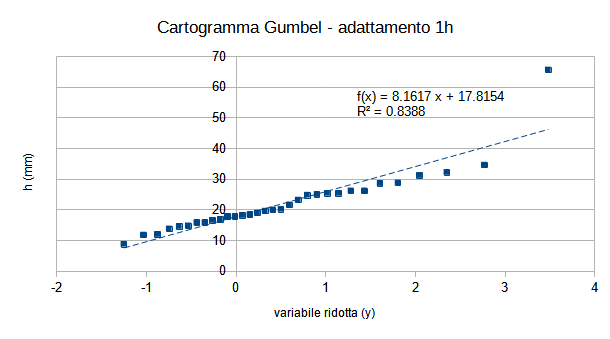
\includegraphics[width=0.7 \textwidth]{immagini/cartogramma_gumbel_1h.png}
    \caption{Cartogramma di Gumbel, con adattamento di precipitazioni di 1 ora di durata.}
    \label{fig:cartogramma_gumbel_1h}
\end{figure}
Il programma con cui è stato ricavato questo grafico (Excel) permette di conoscere la funzione della linea di tendenza, e del relativo valore di $R^2$. \\
Il valore $R^2$, anche detto "Coefficiente di determinazione" è un parametro statistico che permette di misurare il legame tra la variabilità dei dati e la correttezza del modello statistico utilizzato. \cite{r_quadro} \\
Successivamente, è possibile procedere al confronto grafico tra la probabilità empirica P di Weibull e la F(h):
\begin{figure}[H]
    \centering
    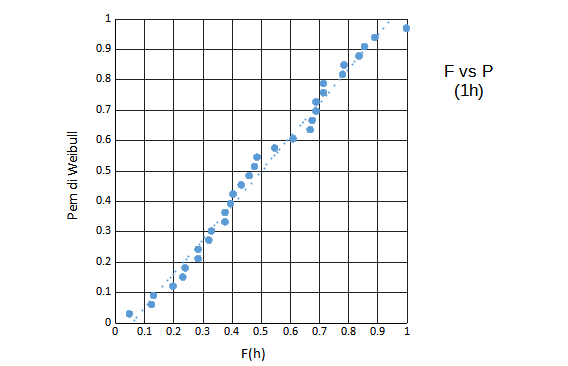
\includegraphics[width=0.7 \textwidth]{immagini/f_vs_p_1h.png}
    \caption{Confronto grafico tra la probabilità empirica di Weibull e la probabilità F(h).}
    \label{fig:f_vs_p_1h}
\end{figure}
La disposizione dei punti attorno la bisettrice permette di intuire come i valori di probabilità siano congruenti reciprocamente.\\
Un altro indicatore con cui è possibile valutare la concordanza di probabilità è il $\chi ^2$. Infatti, tale parametro statistico permette di verificare se le frequenze dei valori osservati si adattano a quelle teoriche, di una distribuzione di probabilità prefissata.\\
Al fine di confermare la coerenza tra le probabilità, il valore del $\chi ^2$ calcolato dev'essere inferiore a quello teorico.\\
Per esempio, nel caso di adattabilità di 1h: 
\begin{itemize}
    \item $\chi ^2$ calcolato: 3.9375
    \item $\chi ^2$ teorico: 5.9915
\end{itemize}
Al fine di conoscere la precipitazione prevista ($h_t$) per un certo tempo di ritorno, occorre valutare la relativa linea segnalatrice di possibilità pluviometrica.\\
Per fare ciò, si utilizzerà la formula 
\begin{equation}
    y_{t}= -\ln \left[ \ln \left(\frac{1}{F(h)} \right) \right] \rightarrow y_{t}= -\ln \left[ \ln \left(\frac{T}{T-1} \right) \right]
    \label{variabile_ridotta}
\end{equation}
Dopo aver trovato il parametro $y_t$, si andrà a ricavare $h_t$ mediante la successiva formula:
\begin{equation}
h_t = u + \alpha \cdot y_t    
\label{h_t}
\end{equation}
Questi calcoli potranno essere ripetuti per ogni fascia oraria disponibile e per qualsiasi tempo di ritorno.\\
Per esempio, la linea segnalatrice di possibilità pluviometrica del nostro bacino, per un tempo di ritorno di 10 anni, è la seguente.
\begin{figure}[H]
    \centering
    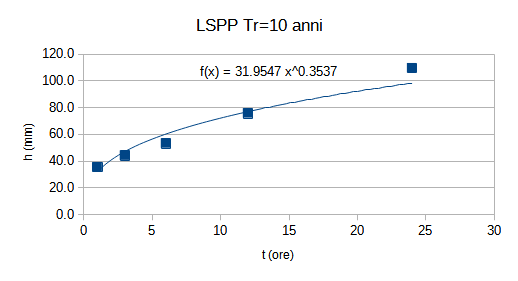
\includegraphics[width=0.7 \textwidth]{immagini/lspp_10anni.png}
    \caption{Linea segnalatrice di probabilità pluviometrica del bacino del fiume Boite, per tempo di ritorno di 10 anni.}
    \label{fig:lspp_10anni}
\end{figure}
Anche per questo caso, il programma che ha permesso il calcolo permette di inserire la funzione matematica della linea di tendenza, che in questo caso è $h_{10}= 31.9547 \cdot x^{0.3537}$. \\
Da tale espressione è possibile conoscere l'altezza di precipitazione di qualsiasi durata (possibilmente inferiore alle 24 ore), per tempo di ritorno di 10 anni. Infatti, nella formula l'incognita è rappresentata dal tempo di durata dell'evento di pioggia.

\subsection{Calcolo della portata di picco}
Lo studio della portata di picco è essenziale per conoscere la massima quantità d'acqua in movimento nel bacino, soprattutto nel caso in cui la durata di un evento pluviometrico eguagli il tempo di corrivazione del bacino.\\
Infatti, è proprio questa la peggiore condizione idraulica, poichè:
\begin{itemize}
    \item all'aumentare della durata di precipitazione l'intensità non aumenta in modo direttamente proporzionale;
    \item al diminuire della durata di precipitazione l'altezza di pioggia è direttamente proporzionale.
\end{itemize}
La funzione che permette di conoscere la portata di picco ($Q_p$) è la seguente:
\begin{equation}
    Q_p = C_d \cdot \frac{h_r \cdot A}{t_c}
    \label{Qp}
\end{equation}
dove: 
\begin{itemize}
    \item $C_d$ è il coefficiente di deflusso;
    \item $h_r(t_c, T_r)$ è l'altezza di pioggia corrispondente al tempo di corrivazione $t_c$ ed al tempo di ritorno $T_r \rightarrow h_r = a \cdot t_c ^n$;
    \item $A$ è l'area del bacino.
\end{itemize}
\subsubsection*{Il tempo di corrivazione}
Il tempo di corrivazione di un bacino ($t_c$) è il tempo massimo che impiega una goccia per attraversare completamente il bacino, fino ad arrivare alla sezione di chiusura.\\
Tale tempo di passaggio può essere calcolato in diversi modo, per questa relazione è stata utilizzata la formula di Giandotti:
\begin{equation}
    t_c = \frac{4 \sqrt{A} + 1.5 \cdot L}{0.8 \cdot \sqrt{z}}
    \label{giandotti}
\end{equation}
dove: 
\begin{itemize}
    \item $A$ è l'area del bacino, in $km^2$;
    \item $L$ è la lunghezza dell'asta principale, in $km$;
    \item $z$ è l'altezza media del bacino rispetto alla sezione di chiusura, espressa in $m$.
\end{itemize}
\subsubsection*{Il coefficiente di deflusso}
Il coefficiente di deflusso è il rapporto tra la precipitazione efficace del bacino e la precipitazione totale. Offre in maniera generale una rappresentazione del deflusso superficiale e dell'infiltrazione del bacino.\\
La formula è quindi:
\begin{equation}
    C_d = \frac{P_e}{h_r}
    \label{Cd}
\end{equation}
\subsubsection*{La precipitazione efficace}
La precipitazione efficace equivale alla quantità d'acqua dell'evento meteorico, al netto delle perdite iniziali e dell'imbibimento del terreno. In pratica è la frazione di precipitazione che si trasforma in deflusso superficiale.\\
Tale valore varia in base alle condizioni del terreno ed in funzione delle caratteristiche del territorio.\\
La formula per calcolare la precipitazione efficace è la seguente: 
\begin{equation}
    P_e = \frac{(h_r - I_a)^2}{h_r - I_a + S}
    \label{Pe}
\end{equation}
dove la lettera $S$ indica lo storage idrico del terreno, che può essere calcolato mediante: 
\begin{equation}
    S = S_0 \cdot \left ( \frac{100}{CN} -1 \right )
    \label{storage}
\end{equation}
Nella precedente funzione, la costante $S_0$ equivale a 254 mm ed il valore CN quantifica la permeabilizzazione del suolo.

\subsection{Progetto della sezione di un canale}
Generalmente, in assenza di vincoli esterni e tecnici, durante il dimensionamento di un canale si adotta la sezione di minima resistenza, ovvero quella sezione che a parità di area permette la velocità media massima, e quindi la portata massima.\\
A parità di altre condizioni, la velocità media dipende dal valore di raggio idraulico (e quindi dalla forma e dimensione della sezione).
\subsubsection*{Calcolo della profondità di moto uniforme $y_1$}
Il parametro $y_1$ indica la profondità del canale con cui la portata $Q$ viene convogliata con la sezione di minor perimetro bagnato.\\
Il calcolo della profondità critica è un metodo iterativo, ovvero il risultato finale si ottiene dalla ripetizione di una serie di calcoli.
Il procedimento inizia con il calcolo di una profondità di primo tentativo $y_0$, mediante la seguente equazione:
\begin{equation}
    y_0 = \left ( \frac{Q}{B \cdot K_S \cdot \sqrt{i_F}} \right) ^ {\frac{3}{5}}
    \label{prof_critica_tentativo}
\end{equation} 
Successivamente si calcola il relativo raggio idraulico, mediante la formula:
\begin{equation}
    Rh_0 = \frac{B \cdot y_0}{B + 2\cdot y_0}
    \label{raggio_idraulico}
\end{equation} 
E da questo raggio idraulico si calcola nuovamente l'altezza $y$:
\begin{equation}
    y_1 = \frac{Q}{B \cdot K_S \cdot R_h ^\frac{2}{3} \cdot \sqrt{i_F}}
    \label{prof_critica}
\end{equation} 
Nel caso che la differenza percentuale tra le due profondità è inferiore al 2\%, il processo può terminare; in caso contrario, occorre ripetere i procedimenti, calcolando il raggio idraulico mediante l'ultima profondità critica ottenuta.
\begin{equation}
    \frac{|y_1 - y_0|}{y_0} \le 2\%
    \label{scostamento_prof_critica}
\end{equation} 
\subsubsection*{Calcolo della $H$ del canale}
Avendo i valori di $y_c$ (calcolata) e di $B$ (di progetto), è possibile calcolare il valore $H$, ovvero l'energia specifica del canale.
La formula per calcolare $H$ è la seguente: 
\begin{equation}
    H = y + \frac{q^2}{2 \cdot g \cdot y^2}
    \label{energia_specifica_canale}
\end{equation} 
Il parametro $q$ indica la portata del canale per unità di larghezza, e si calcola con $q = \frac{Q}{B}$.
\subsubsection*{Calcolo della larghezza limite $B_L$, per il passaggio in condizioni critiche}
Il valore $B_L$, ovvero la larghezza della sezione rettangolare della briglia, in condizioni critiche, si calcola con la seguente formula:
\begin{equation}
    B_L = \frac{Q}{0.414 \cdot \sqrt{g} \cdot H_1 ^{1.5}}
    \label{larghezza_specifica}
\end{equation}